\documentclass[conference]{IEEEtran}
\usepackage[T2A,T1]{fontenc}
\usepackage[utf8]{inputenc}
\usepackage[russian,english]{babel}
\usepackage{booktabs}
\usepackage{amsmath}
\usepackage{graphicx}
\usepackage{url}
\usepackage[hidelinks]{hyperref}
\newcommand{\nViews}{5{,}821{,}987}
\newcommand{\nUsers}{4{,}914}
\newcommand{\nLogChannels}{202}
\newcommand{\labRowsLo}{10.8\%}
\newcommand{\labRowsHi}{11.3\%}
\newcommand{\labAirLo}{16.0\%}
\newcommand{\labAirHi}{16.9\%}
\newcommand{\labRowsTrain}{10.8\%}
\newcommand{\inSlots}{94.1\%}
\newcommand{\inLabSlots}{53.1\%}
\newcommand{\nEvents}{3{,}014{,}129}
\newcommand{\nEventsQ}{615{,}979}
\newcommand{\shareEventsQ}{20.4\%}
\newcommand{\nPairsQ}{230{,}113}
\newcommand{\medProgAny}{249}
\newcommand{\medProgQ}{33}
\newcommand{\nTargetWone}{4{,}349}
\newcommand{\nTargetWtwo}{4{,}030}
\newcommand{\nTestTargetWtwo}{1{,}150}
\newcommand{\tieShare}{67.9\%}
\newcommand{\gapUsers}{23.9\%}
\newcommand{\prevTopMap}{0.3129}
\newcommand{\covQual}{51.2\%}
\newcommand{\covTouched}{65.8\%}
\newcommand{\covAny}{81.0\%}
\newcommand{\testStillAir}{87.9\%}
\newcommand{\nFallbackNone}{4}
\newcommand{\nFallbackFew}{15}
\newcommand{\hsHalfLife}{10}
\newcommand{\hsPrior}{30}
\newcommand{\alsFactors}{32}
\newcommand{\alsAlpha}{1}
\newcommand{\alsReg}{30}
\newcommand{\pprAlpha}{0.5}
\newcommand{\pprWeighting}{count}
\newcommand{\rulesSupport}{30}
\newcommand{\mapHybrid}{0.3612}
\newcommand{\mapHybridTest}{0.3987}
\newcommand{\mapHS}{0.3366}
\newcommand{\mapHScount}{0.3095}
\newcommand{\mapPop}{0.2341}
\newcommand{\mapPPR}{0.3184}
\newcommand{\mapALS}{0.2832}
\newcommand{\mapRules}{0.2545}
\newcommand{\mapContent}{0.0854}
\newcommand{\lbHybrid}{0.45497}
\newcommand{\lbHybridPriv}{0.45015}
\newcommand{\finalFile}{ranker\_v4.csv}
\newcommand{\lbHS}{0.42188}
\newcommand{\lbPop}{0.32330}
\newcommand{\lbPPR}{0.40855}
\newcommand{\diffHS}{0.0246}
\newcommand{\ciHS}{[0.0216, 0.0278]}
\newcommand{\higherHS}{1{,}488}
\newcommand{\lowerHS}{831}
\newcommand{\diffPPR}{0.0428}
\newcommand{\ciPPR}{[0.0394, 0.0463]}
\newcommand{\higherPPR}{1{,}771}
\newcommand{\lowerPPR}{678}
\newcommand{\diffPop}{0.1271}
\newcommand{\ciPop}{[0.1209, 0.1336]}
\newcommand{\higherPop}{2{,}435}
\newcommand{\lowerPop}{713}
\newcommand{\segHybridLight}{0.2385}
\newcommand{\segHSLight}{0.2117}
\newcommand{\segPopLight}{0.1480}
\newcommand{\segHybridHeavy}{0.4845}
\newcommand{\segHSHeavy}{0.4644}
\newcommand{\segPopHeavy}{0.3268}
\newcommand{\mapRankerOneLambda}{0.3566}
\newcommand{\mapEthree}{0.3574}
\newcommand{\mapEfour}{0.3586}
\newcommand{\mapEfourSeeds}{0.3595}
\newcommand{\mapHSfeature}{0.3366}
\newcommand{\impNameA}{the within-user rank of recency-weighted habit coverage}
\newcommand{\impShareA}{33\%}
\newcommand{\impNameB}{the within-user rank of habit-slot exposure}
\newcommand{\impShareB}{17\%}
\newcommand{\impNameC}{the within-user rank of the habit-slot score}
\newcommand{\impShareC}{16\%}
\newcommand{\nFeatures}{80}
\newcommand{\nSeeds}{five}
\newcommand{\nModels}{ten}
\newcommand{\seedRange}{0 to 4}
\newcommand{\rrfK}{0}
\newcommand{\lgbParams}{learning rate 0.02, 63 leaves, 300 rows per leaf, feature fraction 0.5, bagging 0.8, L2 20}
\newcommand{\finalRuntime}{3{,}115}
\newcommand{\mapEfive}{0.3594}
\newcommand{\mapEfiveWide}{0.3597}
\newcommand{\mapFinal}{0.3612}
\newcommand{\nSubmissions}{13}
\newcommand{\hybWatched}{83\%}
\newcommand{\hybNew}{5\%}
\newcommand{\hybPrecFam}{0.434}
\newcommand{\hsPrecFam}{0.397}
\newcommand{\maxPrecNew}{0.157}
\newcommand{\pprWatched}{96\%}
\newcommand{\pprDistinct}{730}
\newcommand{\alsDistinct}{78}
\newcommand{\rulesShared}{3.85}
\newcommand{\rulesNews}{70\%}
\newcommand{\actWatched}{50.9\%}
\newcommand{\actTouched}{14.5\%}
\newcommand{\actNew}{34.6\%}
\newcommand{\actNewRound}{35\%}
\newcommand{\userA}{3525695269081370558}
\newcommand{\hoursA}{350}
\newcommand{\nProgA}{47}
\newcommand{\apHybridA}{0.71}
\newcommand{\apHSA}{0.76}
\newcommand{\apPPRA}{0.64}
\newcommand{\hybListA}{12001682, 12002856, 2400480, 2400508, 2400467}
\newcommand{\hybHitsA}{four}
\newcommand{\hybHitRanksA}{1, 2, 4 and 5}
\newcommand{\hybApFormulaA}{(1/1+2/2+3/4+4/5)/5}
\newcommand{\fillA}{every method filled all five places itself}
\newcommand{\userB}{14049050536217794294}
\newcommand{\hoursB}{59}
\newcommand{\nProgB}{14}
\newcommand{\apHybridB}{0.00}
\newcommand{\apHSB}{0.00}
\newcommand{\apPPRB}{0.00}
\newcommand{\hybListB}{2400467, 2400480, 240081, 500331, 6500479}
\newcommand{\hybHitsB}{no}
\newcommand{\hybHitRanksB}{none}
\newcommand{\hybApFormulaB}{0}
\newcommand{\fillB}{every method filled all five places itself}

% the primitive \input is expandable, so a generated table body can sit between \midrule and \bottomrule
\makeatletter
\newcommand{\tabinput}[1]{\@@input #1 }
\makeatother
\newcommand{\repo}{\url{https://github.com/Marrrik/sweettv-recsys}}

\begin{document}

\title{Habit Meets Schedule: Re-Ranking Five TV\\Programmes per Viewer on sweet.tv}

\author{\IEEEauthorblockN{Mark Starchenko (individual)}
\IEEEauthorblockA{HSE University, Graduate School of Business, mastarchenko@edu.hse.ru, 2026-10-24\\
Final exam quiz: TV programme recommendation on sweet.tv. Code: \repo}}

\maketitle

\begin{abstract}
For 1,260 sweet.tv viewers we predict the five programmes they will most often watch through at least 80\% of an airing in weeks 31 to 42 of 2020, from twenty weeks of channel-level viewing and a broadcast schedule in which only \labRowsTrain{} of rows carry a programme id. We join views to airings by channel and time overlap, rebuild the organisers' target on a weeks 21 to 30 hold-out, and compare popularity, a habit-times-schedule heuristic, implicit ALS, personalised PageRank, association rules and content-based filtering with a LightGBM re-ranker built on all of them. The re-ranker reaches MAP@5 \mapHybrid{} on the hold-out against \mapHS{} for the heuristic and \mapPPR{} for the best single method, and a public score of \lbHybrid{}. Most of the signal is a viewer's own habit placed on the coming schedule, and no method finds the unseen films that light viewers watch next.
\end{abstract}

\begin{IEEEkeywords}
implicit feedback, TV recommendation, learning to rank, personalized PageRank, matrix factorization
\end{IEEEkeywords}

\section{Introduction}
The Kaggle community competition \emph{sweet.tv: TV program recommender}~\cite{kaggle} gives a log of which channel each user watched and when, and the schedule of what aired. The data page defines the target: per user and airing compute the watched share, keep airings watched for at least 0.8 of their length, count them per programme, and take strictly the five most frequent programmes of weeks 31 to 42, ranked by MAP@5. The quiz requires at least two of four method families, a popularity reference, one documented hold-out and a strategy a service could adopt.

A TV service needs such a list for a ``your programmes'' row: what to remind a viewer of, and what new to show. The task is unusual because the items are scheduled: a programme can only be watched when it airs, and the schedule of the test weeks is public.

\emph{Example.} User A (test user \userA) fully watched \emph{SpongeBob SquarePants} on 32 airings, a second cartoon on 16 and the \emph{TSN} news on 10 in weeks 11 to 20. The hybrid, trained on earlier snapshots, returns ids 12001682, 12002856, 2400480, 2400508, 2400467 for weeks 21 to 30; four of them are in A's actual top five (AP@5 \apHybridA).

\emph{Contributions.} (1) A leak-free reconstruction of the target on time snapshots, with a heuristic that multiplies a user's per-airing watch rate by the airings in the coming schedule. (2) A comparison of six single methods and a re-ranker on one hold-out with paired bootstrap intervals, and an account of which list properties explain the differences.

\section{Related Work}
Hu, Koren and Volinsky~\cite{hu2008} built implicit-feedback ALS for exactly this setting, a TV service where $r_{ui}$ counts how many times a user fully watched a show, with confidence $c_{ui}=1+\alpha\log(1+r_{ui}/\epsilon)$ as one variant; they note that predicting a re-watch is much easier than a first watch. Personalised PageRank restarts a random walk at a user-specific preference vector~\cite{jeh2003}. Association rules score $X\Rightarrow Y$ by support and confidence~\cite{agrawal1993}. Two-stage systems first generate a few hundred candidates and then rank them with a richer model~\cite{covington2016}. LambdaMART is the boosted-tree version of LambdaRank~\cite{burges2010}; we use the gradient boosting library LightGBM~\cite{ke2017} and its \texttt{lambdarank} objective. Reciprocal rank fusion sums $1/(k+r)$ over rankings, with $k=60$ fixed by its authors~\cite{cormack2009}.

\emph{Alternatives considered.} Sequence models over the view stream: the target counts repeated full viewings, which a per-airing rate already captures, at a fraction of the cost. Recovering programme ids for unlabelled airtime by title: only 4.4\% of unlabelled airtime has a title equal to a labelled one (EDA), so it would add little. A neural two-tower retriever: the candidate stage already covers 78.6\% of target pairs with simple sources.

\section{Method}
\subsection{Join, watched rule and unlabelled airtime}
A view matches every schedule slot on the same channel (\texttt{vsetv\_id} equals \texttt{channel\_id}) whose airing interval overlaps the view; the covered seconds of one airing are summed over the user's views and divided by the slot length, capped at 1. The 0.8 threshold is the organisers' rule, so our labels and our test target are defined the same way. The observed distribution supports a share-based cut over an absolute one: covered shares are bimodal (Fig.~\ref{fig:data}b), and 71\% of events on slots of at most 10 minutes reach 0.8 against 7\% on slots over two hours, so a fixed number of seconds would mean very different things for news and films. Rows with \texttt{tv\_show\_id}~=~0 are not items: they never enter the pool or the targets, but all airtime, labelled or not, feeds the viewing-habit features below. The two clocks agree: view stops cluster at slot boundaries only at zero shift, in every week.

\begin{figure}[t]
\centering
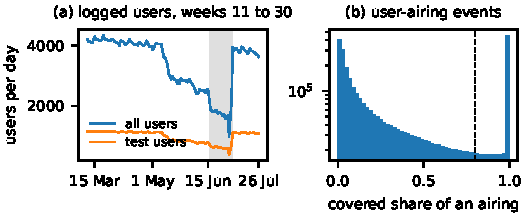
\includegraphics[width=\columnwidth]{fig_data.pdf}
\caption{(a) Users with a view per day; shaded: 16 June to 4 July, \gapUsers{} of users active before and after have no view inside it, and 3 July is empty. (b) Covered share of \nEvents{} user-airing events, log scale; dashed: the 0.8 rule (\texttt{report/make\_figures.py}).}
\label{fig:data}
\end{figure}

\subsection{Snapshots, hold-out and leakage}
A snapshot $S_T$ uses views before Monday of ISO week $T$, clipped at that moment, as history, and the target of weeks $T$ to the window end. The hold-out is $S_{21}$ (history weeks 11 to 20, target 21 to 30, \nTargetWtwo{} users, \nTestTargetWtwo{} of them test users): it is the latest window the quiz allows, adjacent to the test window and close to it in length (10 weeks against 12), and its history has the same start as the final model's. Every model is refitted per snapshot on its history only; the target-window schedule tells which programme airs where and when, never who watched it. The ranker learns from $S_{14}$, $S_{16}$ and $S_{18}$, whose labels end in week 20, with early stopping on 20\% of their users, so $S_{21}$ is used only to choose. The final models are refitted on $S_{14}$, $S_{16}$, $S_{18}$, $S_{21}$ and $S_{26}$ and predict $S_{31}$ (history 11 to 30, target 31 to 42).

\subsection{Common rules for every method}
The pool is the labelled programmes that air in the target window; recommending an already watched programme is allowed for every method. A method's positive scores are sorted (ties by id) and the empty places are filled from one popularity ranking, the same for all methods and the whole answer for users without history: pool programmes ordered by how many users have them in their history top five, then by airings in the window. Among test users \nFallbackNone{} have no fully watched airing in weeks 11 to 30 and get this list, and \nFallbackFew{} have one to four such programmes and get it after their own. Every list therefore has exactly five distinct ids. Scores of different methods are never compared directly.

\subsection{Single methods}
\emph{Popularity} is that fallback ranking alone. \emph{Habit $\times$ schedule} scores
\[
s(u,p)=\sum_{c}\min\Bigl(1,\frac{q_w(u,p,c)}{e_w(u,p,c)+\pi}\Bigr)\,A(p,c),
\]
where $q_w$ counts the airings of $p$ on channel $c$ that $u$ watched for 0.8, $e_w$ the airings of $p$ on $c$ on days $u$ was in the log (both weighted with a \hsHalfLife-week half-life), $\pi=\hsPrior$ and $A$ the airings of $p$ on $c$ in the window. Counting only logged days keeps rates comparable across the logging gap of Fig.~\ref{fig:data}a. \emph{ALS} follows~\cite{hu2008} with $c=1+\alpha\log(1+w)$, $w$ the recency-weighted count, \alsFactors{} factors, $\alpha=\alsAlpha$, $\lambda=\alsReg$, 15 sweeps of the closed-form solves. \emph{PPR} walks a programme graph whose edge weight is the number of users who fully watched both programmes, row-normalised, follows an edge with probability \pprAlpha{} and restarts at the user's normalised $\log(1+w)$ history. \emph{Association rules} score $C$ by $\max_{A}P(C\mid A)$ over the user's programmes $A$, for pairs shared by at least \rulesSupport{} users. \emph{Content-based} builds TF-IDF vectors from category, genres, decade, directors and actors and ranks by cosine similarity to the user's weighted profile.

\subsection{Hybrid: candidates and re-ranking}
Candidates are every pool programme the user touched in the history, the top 60 of popularity, ALS, PPR, rules and of a habit-slot score, and the top 20 of content. The habit-slot score multiplies a user's share of each channel and hour of the week spent watching (all airtime) by the airings a programme has in those cells. The ranker sees 67 features: the habit $\times$ schedule score and two variants, counts, rates and recency of the user's views of the programme, window and history airings, habit-slot exposure with each airing spread over all the hours it covers, programme popularity, category and year, user activity, every method's score and its rank within the user. Labels mark membership in the target five. LightGBM~4.7.0 is trained with the binary and the \texttt{lambdarank} objectives (one group per user and snapshot) and three seeds; the six models are fused by summing $1/\mathrm{rank}$ within the user, which is reciprocal rank fusion~\cite{cormack2009} with $k=0$ instead of its authors' $60$. Weights are equal and not tuned.

\subsection{Configuration}
LightGBM: learning rate 0.03, 31 leaves, 300 rows per leaf, feature fraction 0.6, bagging 0.8, L2 10, final rounds 1.2 times the early-stopping optimum. Seeds: 0 for ALS, sampling and bootstrap, 0 to 2 for LightGBM. Environment: Windows 11, AMD Zen~4 laptop CPU (16 threads), 15.2~GB RAM, Python 3.12.14, NumPy 2.5.4, pandas 3.0.6, SciPy 1.18.1, scikit-learn 1.9.1. Runtimes: EDA 72~s, single methods 215~s, final re-ranker notebook 1,488~s including all six snapshots.

\section{Experiments}
\subsection{Setup}
The log holds \nViews{} views of \nUsers{} users on \nLogChannels{} channels from 9 March to 26 July 2020; \labRowsLo{} to \labRowsHi{} of schedule rows and \labAirLo{} to \labAirHi{} of airtime carry an id. \inSlots{} of viewing time falls inside some slot and \inLabSlots{} inside labelled slots. Of \nEvents{} user-airing events, \nEventsQ{} (\shareEventsQ) reach 0.8. MAP@5 is averaged over the hold-out target users; differences use a paired bootstrap over users (2,000 resamples). Kaggle scores are the returned late-submission scores.

\begin{table*}[t]
\centering
\caption{Single methods and the final hybrid. MAP@5 on the hold-out $S_{21}$ (all \nTargetWtwo{} target users, and the \nTestTargetWtwo{} test users among them), on $S_{16}$ (history weeks 11 to 15, target 16 to 20), and the returned Kaggle scores. Last column: hybrid minus method on $S_{21}$ with a 95\% paired bootstrap interval (\texttt{modelling/analysis.ipynb}).}
\label{tab:methods}
\begin{tabular}{lrrrrrr}
\toprule
Method & $S_{21}$ all & $S_{21}$ test users & $S_{16}$ all & public & private & hybrid $-$ method on $S_{21}$ \\
\midrule
\tabinput{generated/tab_methods.tex}
\bottomrule
\end{tabular}
\end{table*}

\subsection{Results}
Table~\ref{tab:methods} compares the methods. Habit $\times$ schedule beats every single method and beats the count of fully watched airings alone (\mapHScount) by 0.027; the hybrid beats it by \diffHS{} \ciHS{}, higher for \higherHS{} users and lower for \lowerHS{}. The order of the methods is the same on $S_{21}$, on $S_{16}$ and on the public score. Kaggle scores are higher than hold-out scores for every method; the test window is longer (12 weeks against 10) and has no logging gap, which we take as the likely reason without having tested it.

Table~\ref{tab:ranker} traces the re-ranker. Larger candidate lists raised recall of the target from 75.7\% to 78.6\% but not MAP@5; more training snapshots and stronger regularisation gave +0.002, coverage features +0.001 and three seeds +0.001. Each step is within the noise of a single run, but together they moved both $S_{21}$ and the public score. The largest gain shares in the final model are \impNameA{} (\impShareA), \impNameB{} (\impShareB) and \impNameC{} (\impShareC).

\begin{table}[t]
\centering
\caption{Re-ranker rounds: training snapshots, candidate top-$n$ (sources/popularity), features, objectives (b+l: binary and lambdarank), MAP@5 on $S_{21}$ and public score of the submitted ones (\texttt{modelling/ranker*.ipynb}).}
\label{tab:ranker}
\setlength{\tabcolsep}{2.2pt}
\footnotesize
\begin{tabular}{lllllrrr}
\toprule
Round & Train & Cand. & Feat. & Objective & all & test & public \\
\midrule
\tabinput{generated/tab_ranker.tex}
\bottomrule
\end{tabular}
\end{table}

\begin{table}[t]
\centering
\caption{Properties of the top-5 lists on $S_{21}$: share of recommended programmes the user watched for 0.8 before, only touched, or never touched; precision on familiar and on new programmes; distinct programmes over all users; mean overlap with the popularity five; share of news. In the actual targets 50.9\% / 14.5\% / 34.6\% are watched / touched / new.}
\label{tab:props}
\setlength{\tabcolsep}{2pt}
\footnotesize
\begin{tabular}{lrrrrrrrr}
\toprule
Method & watch. & touch. & new & P fam. & P new & dist. & pop. & news \\
\midrule
\tabinput{generated/tab_props.tex}
\bottomrule
\end{tabular}
\end{table}

\begin{table*}[t]
\centering
\caption{Top 5 of every method on $S_{21}$ for users A (\userA, \hoursA{} labelled hours and \nProgA{} fully watched programmes in weeks 11 to 20) and B (\userB, \hoursB{} hours, \nProgB{} programmes), chosen before any list was seen as the test users closest to the 90th percentile of labelled hours and to the 10th percentile among those with at least one fully watched airing. Bold: in the actual top five of weeks 21 to 30. No mark: watched for 0.8 before; $t$: only touched; $n$: never touched. Last column of each block: AP@5. For A \fillA; for B \fillB. Titles and categories from the schedule are listed below the table; the test-window lists are in \texttt{modelling/analysis.ipynb}.}
\label{tab:users}
\scriptsize
\setlength{\tabcolsep}{2.5pt}
\begin{tabular}{l*{5}{r}r@{\hspace{8pt}}*{5}{r}r}
\toprule
 & \multicolumn{6}{c}{User A} & \multicolumn{6}{c}{User B} \\
Method & 1 & 2 & 3 & 4 & 5 & AP & 1 & 2 & 3 & 4 & 5 & AP \\
\midrule
\tabinput{generated/tab_users.tex}
\bottomrule
\end{tabular}
\par\smallskip
\parbox{\textwidth}{\scriptsize\raggedright 20088 \foreignlanguage{russian}{'Завтрак с 1+1'. Информационно-развлекательная программа} (entertainment); 240081 \foreignlanguage{russian}{Факты. День} (news); 400335 \foreignlanguage{russian}{'Хата на тата', 7 сезон, 1 эп} (entertainment); 400361 \foreignlanguage{russian}{'МастерШеф', 7 сезон, 17 эп} (factual); 500331 \foreignlanguage{russian}{'Один за всех'} (entertainment); 1000381 \foreignlanguage{russian}{Т/с 'CSI: Место преступления', 7 сезон, 6 и 7 с} (series); 1100411 \foreignlanguage{russian}{Премьера. 'Вещдок. Особый случай. Око за око'} (factual); 2400467 \foreignlanguage{russian}{'Викна-Новости'} (news); 2400480 \foreignlanguage{russian}{'ТСН. Неделя'} (news); 2400508 \foreignlanguage{russian}{Сегодня. Итоги с Олегом Панютой} (news); 2500413 \foreignlanguage{russian}{Гражданская оборона} (news); 5900319 \foreignlanguage{russian}{Абзац!} (news); 5900347 \foreignlanguage{russian}{'Деньги'} (news); 10002893 \foreignlanguage{russian}{Т/с 'Когда мы дома'} (series); 10003012 \foreignlanguage{russian}{Т/с 'Однажды в Одессе'} (series); 12001682 \foreignlanguage{russian}{М/с 'Губка Боб Квадратные Штаны'} (kids); 12001734 \foreignlanguage{russian}{М/с 'Волшебные покровители', 154 с. 'Хочу это вырезать / Мэрский день'} (kids); 12002720 \foreignlanguage{russian}{М/с 'Соник Бум'} (kids); 12002856 \foreignlanguage{russian}{М/с 'Элвин и бурундуки'} (kids); 12002904 \foreignlanguage{russian}{М/с 'Рыцари Нексо Найтс'} (kids); 90055475 \foreignlanguage{russian}{Х/ф 'Парк Юрского периода 3'} (film); 90057266 \foreignlanguage{russian}{Х/ф 'Терминатор 3: Восстание машин'} (film); 90072084 \foreignlanguage{russian}{Х/ф 'РЭД'} (film); 90082736 \foreignlanguage{russian}{Х/ф 'Человек-паук. Вдали от дома'} (film); 120079707 \foreignlanguage{russian}{М/ф 'Король обезьян'} (kids); 120082346 \foreignlanguage{russian}{М/ф 'Муми-тролли и зимняя сказка'} (kids).
}
\end{table*}

\subsection{Recommendation examples}
Table~\ref{tab:users} shows the same two users for all methods. A watches cartoons and news; habit $\times$ schedule finds four of A's five (AP \apHSA), the hybrid four in a different order (\apHybridA) and PPR four (\apPPRA). B's actual five are four films B never touched and the series \emph{CSI}, watched once before; every method scores 0, and only content-based and rules propose anything new, all of it wrong.

\subsection{Verification}
\texttt{tests/check\_core.py} checks AP@5 against hand-computed cases (hits at ranks 1 and 2 of five give 0.4, at ranks 4 and 5 give 0.13), the join on a toy schedule, the target rule, one ALS half-step against eq.~(4) of~\cite{hu2008} written out directly, and that every submission has the template's 1,260 users in the template's order with five distinct ids. The second round was repeated inside the third with the same seeds and gave the same $S_{21}$ values to four decimals. Kaggle accepted every file and returned the scores of Table~\ref{tab:methods}, read back with the Kaggle CLI.

\begin{figure}[t]
\centering
\IfFileExists{kaggle_score.png}{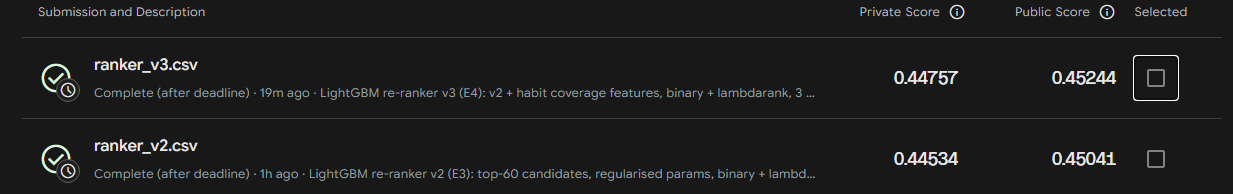
\includegraphics[width=\columnwidth]{kaggle_score.png}}{\fbox{\parbox{0.9\columnwidth}{\centering\vspace{1.2cm}[AUTHOR: screenshot of the Kaggle submissions page with \texttt{ranker\_v3.csv}, public score \lbHybrid]\vspace{1.2cm}}}}
\caption{Returned Kaggle score of the designated final submission \texttt{ranker\_v3.csv}.}
\label{fig:kaggle}
\end{figure}

\section{Discussion}
\subsection{Which strategy should the platform select?}
On the hold-out the hybrid has the best MAP@5 (\mapHybrid) and the best public score (\lbHybrid). It beats habit $\times$ schedule by \diffHS{} \ciHS{} and PPR by \diffPPR{} \ciPPR{} (Table~\ref{tab:methods}). Most of the gain comes from a better order of programmes the user already watches. The hybrid has the highest precision on familiar programmes (Table~\ref{tab:props}), 83\% of its slots are programmes the user watched before and only 5\% are new to the user, while 35\% of the actual targets are new. Habit $\times$ schedule needs no training and scores \lbHS{} on the public board. Light users are hard for every method: on $S_{21}$ the hybrid scores \segHybridLight{} on the lightest third of users and \segHybridHeavy{} on the heaviest.

We read these numbers as follows; none of the explanations was tested by a decomposition. The target counts repeated full viewings, so it is dominated by programmes that air often and that the user already finishes. \emph{TSN} is in the target five of half of the hold-out users, and news make 28\% of target pairs against 2.6\% of labelled airtime (EDA). This is why popularity alone reaches \mapPop{}, and why association rules mostly find the same programmes again (on average 3.85 of their 5 are in the popularity five, and 70\% are news): a rule from one news programme to another has high confidence for almost every user. ALS pulls the user towards what similar users finish. With the strong regularisation selected on the hold-out it recommends only 78 distinct programmes and loses the user's smaller habits, which is where it falls behind PPR. PPR keeps half of the walk's mass on the user's own history, so 96\% of its slots are familiar. The diffusion then orders those programmes by co-viewing centrality, while habit $\times$ schedule orders them by how often the user finishes them; this costs PPR against habit $\times$ schedule but gives it the widest catalogue coverage (730 programmes). Content attributes describe films well, but the target is mostly news and cartoons. Among new target programmes the user's favourite category matches 23.1\% of the time, against 21.6\% expected from category popularity alone (EDA), so content-based comes last. The schedule matters because a programme that stops airing cannot be watched: in the EDA, no top-five programme that stopped airing stayed in the next target.

We propose to serve the hybrid as the personalised ``your programmes'' row and to keep habit $\times$ schedule as the fallback when the model is unavailable. The current lists should not be presented as discovery. An unfamiliar programme in them is mostly a wrong guess (precision on new programmes is at most 0.157), and nothing here shows whether a viewer would enjoy it. A separate row with premieres in the viewer's usual channels and hours could be tested online; we have not measured it. The cost is low at this scale: the final notebook builds candidates and features for six snapshots and trains all models in 1,488~s on a laptop.

\subsection{Failure case}
The first table of list properties reported for habit $\times$ schedule ``share watched at 0.8 before 0.0025, share new to the user 0.9975''. A method that recommends almost only watched programmes cannot have these values, and user A's \emph{SpongeBob}, watched 32 times, was marked ``new''. The cause was in how the sets of (user, programme) pairs were built: \texttt{DataFrame.to\_numpy()} over a \texttt{uint64} and an \texttt{int64} column returns \texttt{float64}, because NumPy promotes the two types to a common one. Twenty-digit user ids exceed $2^{53}$, so they were rounded and never matched. We now build the pairs from \texttt{zip(col.tolist())}. After the fix the share is 0.958, A's programmes are marked watched, and MAP@5, which is computed on another path, is unchanged. An earlier failure affected only the run time. The first ALS grid used over two hours of CPU without finishing, because a multi-threaded BLAS spent its time switching threads on one $64\times64$ solve per user. With BLAS limited to one thread a fit takes 4 to 47~s.

\subsection{What worked, what surprised, limitations}
Three things worked: rebuilding the organisers' target exactly, scoring by the expected airings in the coming schedule, and the habit-slot features, which carry most of the ranker's gain. We did not expect content-based to fall so far below popularity or more candidates to bring no gain, and we did not expect the public score to be 0.08 to 0.09 above the hold-out for every method except content-based. The main limitation is that only \labRowsTrain{} of schedule rows carry an id, so news and shows aired under unlabelled titles can be neither recommended nor counted. The hold-out target comes from a log with a gap that affects \gapUsers{} of users. \tieShare{} of hold-out users have a tie between places five and six, and the organisers do not say how ties are broken, so part of the target is noise to every method. A programme missing from this log may still have been seen elsewhere. All results are offline and come from one platform and one season.

\subsection{Next improvement}
Instead of the linear coverage sums used now, predict for each user and airing the probability of covering 0.8 of it from the user's channel-hour habits, and sum these probabilities over the window's airings. The coverage features are already the strongest predictors, and their linear form ignores that a two-hour film needs almost all of its hours covered.

\section{AI Usage Disclosure}
\subsection{AI tools}
Claude Opus 5.5 (\texttt{claude-opus-5-5}) in Claude Code 2.1.304, VS Code extension.

\subsection{How AI was used}
\emph{Code:} all of \texttt{src/}, the notebooks, \texttt{tools/}, \texttt{tests/} and the report scripts. \emph{Analysis and runs:} EDA, every experiment, Kaggle submissions with the CLI. \emph{Debugging:} the failures of Section~V-B and the Windows process issues. \emph{Search and reading:} the competition data page, the course guidelines and the cited papers. \emph{Drafting:} the whole text of this report.

\subsection{What I personally verified}
I hand-computed AP@5 of user A for the hybrid from Table~\ref{tab:users}: the hits are at ranks 1, 2, 4 and 5, so AP@5 $=(1/1+2/2+3/4+4/5)/5=\apHybridA$, the value in the table. On the Kaggle submissions page \texttt{ranker\_v3.csv} shows a private score of \lbHybridPriv{} and a public score of \lbHybrid{}, as in Table~\ref{tab:methods}; Fig.~\ref{fig:kaggle} is my screenshot of that page. I ran \texttt{python tests/check\_core.py}, and every check printed ``ok'', including the format check of all 12 submission files. I checked that \texttt{modelling/baselines.ipynb} reports MAP@5 \mapPop{} for popularity and \mapHS{} for habit $\times$ schedule on $S_{21}$, as in Table~\ref{tab:methods}. I opened the DOIs of~\cite{hu2008,jeh2003,agrawal1993,covington2016,cormack2009} and the links of~\cite{ke2017,burges2010,kaggle}; authors, venues and years match the reference list.

\subsection{What I trusted without verification}
The join was checked on a toy schedule and by the clock-alignment test, not line by line on real data. I checked the bibliographic records of all references but did not read the papers myself; in the session the AI read the text of~\cite{hu2008,cormack2009,covington2016} and only the records or publisher pages of the others. We read the data page's ``screen time'' as a share per airing; a share per programme would change the target. The test window and its target are hidden, so all statements about weeks 31 to 42 rest on the returned scores.

\subsection{Session log reference}
The attached session export is the unmodified log of the Claude Code session in which this work was done.

\begin{thebibliography}{8}
\bibitem{hu2008} Y. Hu, Y. Koren, and C. Volinsky, ``Collaborative filtering for implicit feedback datasets,'' in \emph{Proc. 8th IEEE Int. Conf. Data Mining (ICDM)}, 2008, pp. 263--272, doi: 10.1109/ICDM.2008.22.
\bibitem{jeh2003} G. Jeh and J. Widom, ``Scaling personalized web search,'' in \emph{Proc. 12th Int. Conf. World Wide Web (WWW)}, 2003, doi: 10.1145/775152.775191.
\bibitem{agrawal1993} R. Agrawal, T. Imieli\'nski, and A. Swami, ``Mining association rules between sets of items in large databases,'' in \emph{Proc. ACM SIGMOD Int. Conf. Management of Data}, 1993, pp. 207--216, doi: 10.1145/170035.170072.
\bibitem{ke2017} G. Ke \emph{et al.}, ``LightGBM: A highly efficient gradient boosting decision tree,'' in \emph{Advances in Neural Information Processing Systems 30 (NIPS)}, 2017. [Online]. Available: \url{https://papers.nips.cc/paper_files/paper/2017/hash/6449f44a102fde848669bdd9eb6b76fa-Abstract.html}
\bibitem{covington2016} P. Covington, J. Adams, and E. Sargin, ``Deep neural networks for YouTube recommendations,'' in \emph{Proc. 10th ACM Conf. Recommender Systems (RecSys)}, 2016, pp. 191--198, doi: 10.1145/2959100.2959190.
\bibitem{burges2010} C. J. C. Burges, ``From RankNet to LambdaRank to LambdaMART: An overview,'' Microsoft Research, Tech. Rep. MSR-TR-2010-82, 2010. [Online]. Available: \url{https://www.microsoft.com/en-us/research/publication/from-ranknet-to-lambdarank-to-lambdamart-an-overview/}
\bibitem{cormack2009} G. V. Cormack, C. L. A. Clarke, and S. Buettcher, ``Reciprocal rank fusion outperforms Condorcet and individual rank learning methods,'' in \emph{Proc. 32nd Int. ACM SIGIR Conf.}, 2009, pp. 758--759, doi: 10.1145/1571941.1572114.
\bibitem{kaggle} sweet.tv, ``sweet.tv --- TV program recommender,'' Kaggle community competition, 2020. [Online]. Available: \url{https://www.kaggle.com/competitions/sweettv-tv-program-recommender}. [Accessed: 2026-10-21].
\end{thebibliography}

\end{document}
